As stated in the previous section, the solution focuses on implementing 
the ECB and CBC algorithms in the Atmega controller firmware along with a series 
of optimizations meant to keep power consumption at a minimum.

\subsection{ECB and CBC algorithms}

Both the ECB and CBC algorithms represent block ciphers. These algorithms operate 
on fixed-length groups of bits called blocks. In order to encrypt/decrypt a block 
of data, a key is necessary. The difference between the two methods lies in how 
the key is applied.

For the ECB mode, each block is encrypted separately with the respective key, as 
show in the figure below. The disadvantage of this method is that identical plain text 
blocks shall generate identical cipher text blocks, which allows data patterns to 
emerge, thus making this encryption method relatively vulnerable to attacks.

\begin{figure}[ht] \centering
  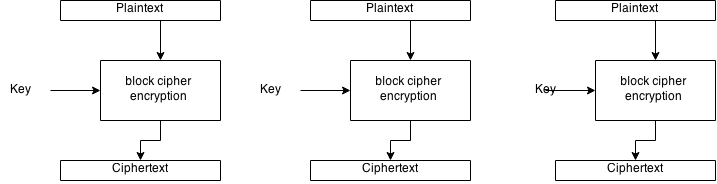
\includegraphics[width=0.5\textwidth]{img/ECB-function-mode.png}
  \caption{ECB mode of operation}
\end{figure}

In contrast, CBC mode encrypts a block by using information from either the previous 
block, or and initialization vector (IV). A XOR operation is performed between the 
plain text and the previous cipher text or IV before applying the key. This method 
ensures pseudo-randomness and prevents patterns from emerging, thus making it 
more resilient to attacks.

\begin{figure}[ht] \centering
  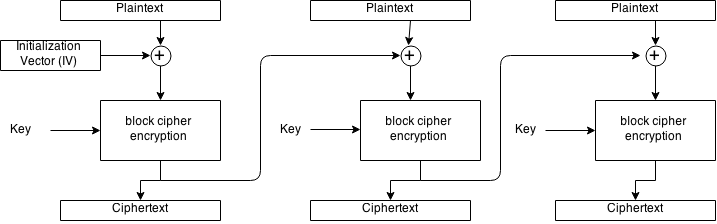
\includegraphics[width=0.5\textwidth]{img/CBC-function-mode.png}
  \caption{CBC mode of operation}
\end{figure}

\subsection{Disadvantages of key based algorithms}

There are two main reasons why the chosen encryption method is ECB/CBC. The first 
reason is that when ported to a different architecture which incorporates the 
transceiver on the same chip as the controller, the encryption and decryption can be safely 
handed over to the AES with minimal modifications and almost no degradation in 
power consumption.

The second reason is that an alternative solution would represent using key based 
encryption methods (both symmetric and asymmetric). Amongst the downsides of this 
particular method, we are mainly concerned with the following:

\begin{itemize}

\item Increased power consumption. Due to the nature and complexity of these algorithms 
as well as the number of operations which must be performed, the cost of such a 
solution is not optimal for low power sensors. By cost we refer to the necessary 
processing power and the total power consumption of the wireless sensor node.
\item Memory limitations. The wireless sensor nodes were not designed to support 
external flash memory modules. The only available memory is the ATmega controller's 
flash memory. Since this memory is limited, writing additional data in it such as 
the node's private key and the public keys of other nodes would not be practical.
A possible solution would be to add a special type of node which handles all data 
decryption and verification on the path towards the base station, but this would 
increase the size and complexity of the network.
\item Key vulnerability. There are situations in which nodes will have to transmit 
public keys between themselves. Unless the respective keys are also encrypted prior 
to sending, should a man-in-the-middle type of attack occur, the keys can be intercepted 
and thus compromise the security of future transmissions.

\end{itemize}

\subsection{Optimizations}

Despite being a more efficient technique from a power consumption point of view, the 
software implementation can be improved even further by reducing the number of operations 
that must be performed on the microcontroller.

In the wireless sensor network, each node is identified by a MAC. In order to optimize the 
operations performed by a node when it receives a packet and also prevent attacks which 
try to introduce corrupt packets in the network, it shall first check if the source MAC 
is valid. This additional layer of security is cheap to implement and versatile.

First, each node shall contain a table of valid MACs stored in its local flash. The size of this 
table is proportional to the number of sensors in the network. Once a node has this table, upon 
receiving a packet, it shall drop it unless the source MAC matches an entry in the table 
and no decryption and verification operations shall be initiated.

Another software optimization is related to data processing before packets are assembled and 
the encryption operation can effectively begin. The data provided by the main sensor, the 
accelerometer, is often of no interest, as it presents no immediate changes in the frequency of 
an object's vibrations. Thus, in order to reduce the number of packets which a sensor node sends 
and prevent the flooding of the communication channel, this data is pre-processed.

Once the network is assembled and the nodes are powered on, they shall take a set of 
readings in order to calibrate themselves to a certain level of vibrations. Then, 
whenever input is provided from the accelerometer, if that specific input is in 
range of the default values obtained during calibration, the information is dropped 
and no packet is formed. Furthermore, relevant data which is not in the range of the 
normal values is not sent after every reading. Instead, a series of N such readings 
from the accelerometer are processed into a median value, which is then transmitted 
into the network. Using this technique, the controller processes more useful information 
and the network will not flood itself.
